\chapter{Rigid-fluid coupling}
\label{chap:rfc}
We model the dynamics of rigid bodies and the coupled behavior of fluid and
rigid bodies. Transport of arbitrarily shaped rigid bodies in fluid flows is a
common phenomenon that occurs widely in nature. We couple CTVF with DEM to
handle the rigid fluid coupling problems. The fluid phase is modeled using a
corrected transport velocity formulation. CTVF provides smooth pressure
distribution with EDAC formulation and homogeneous particle distribution,
resulting in accurate fluid modeling. Rigid-rigid interactions are modeled with
DEM. The interaction between the fluid phase and rigid bodies is handled using
the dummy particle approach.

We consider the sliding of a rigid body to demonstrate the rigid-rigid interaction
modeling. A rigid body is allowed to slide on a frictional surface.
\Cref{fig:results-solid-sliding-velocity-vs-time-2d} shows a evolution of
velocity of the center of mass of the rigid body for different frictional
coefficients against the analytical solution. From
\cref{fig:results-solid-sliding-velocity-vs-time-2d} we can see that the current
solver has an excellent match with the analytical solution and covers all the
regimes of the sliding case.
\begin{figure}[tpb]
  \centering
  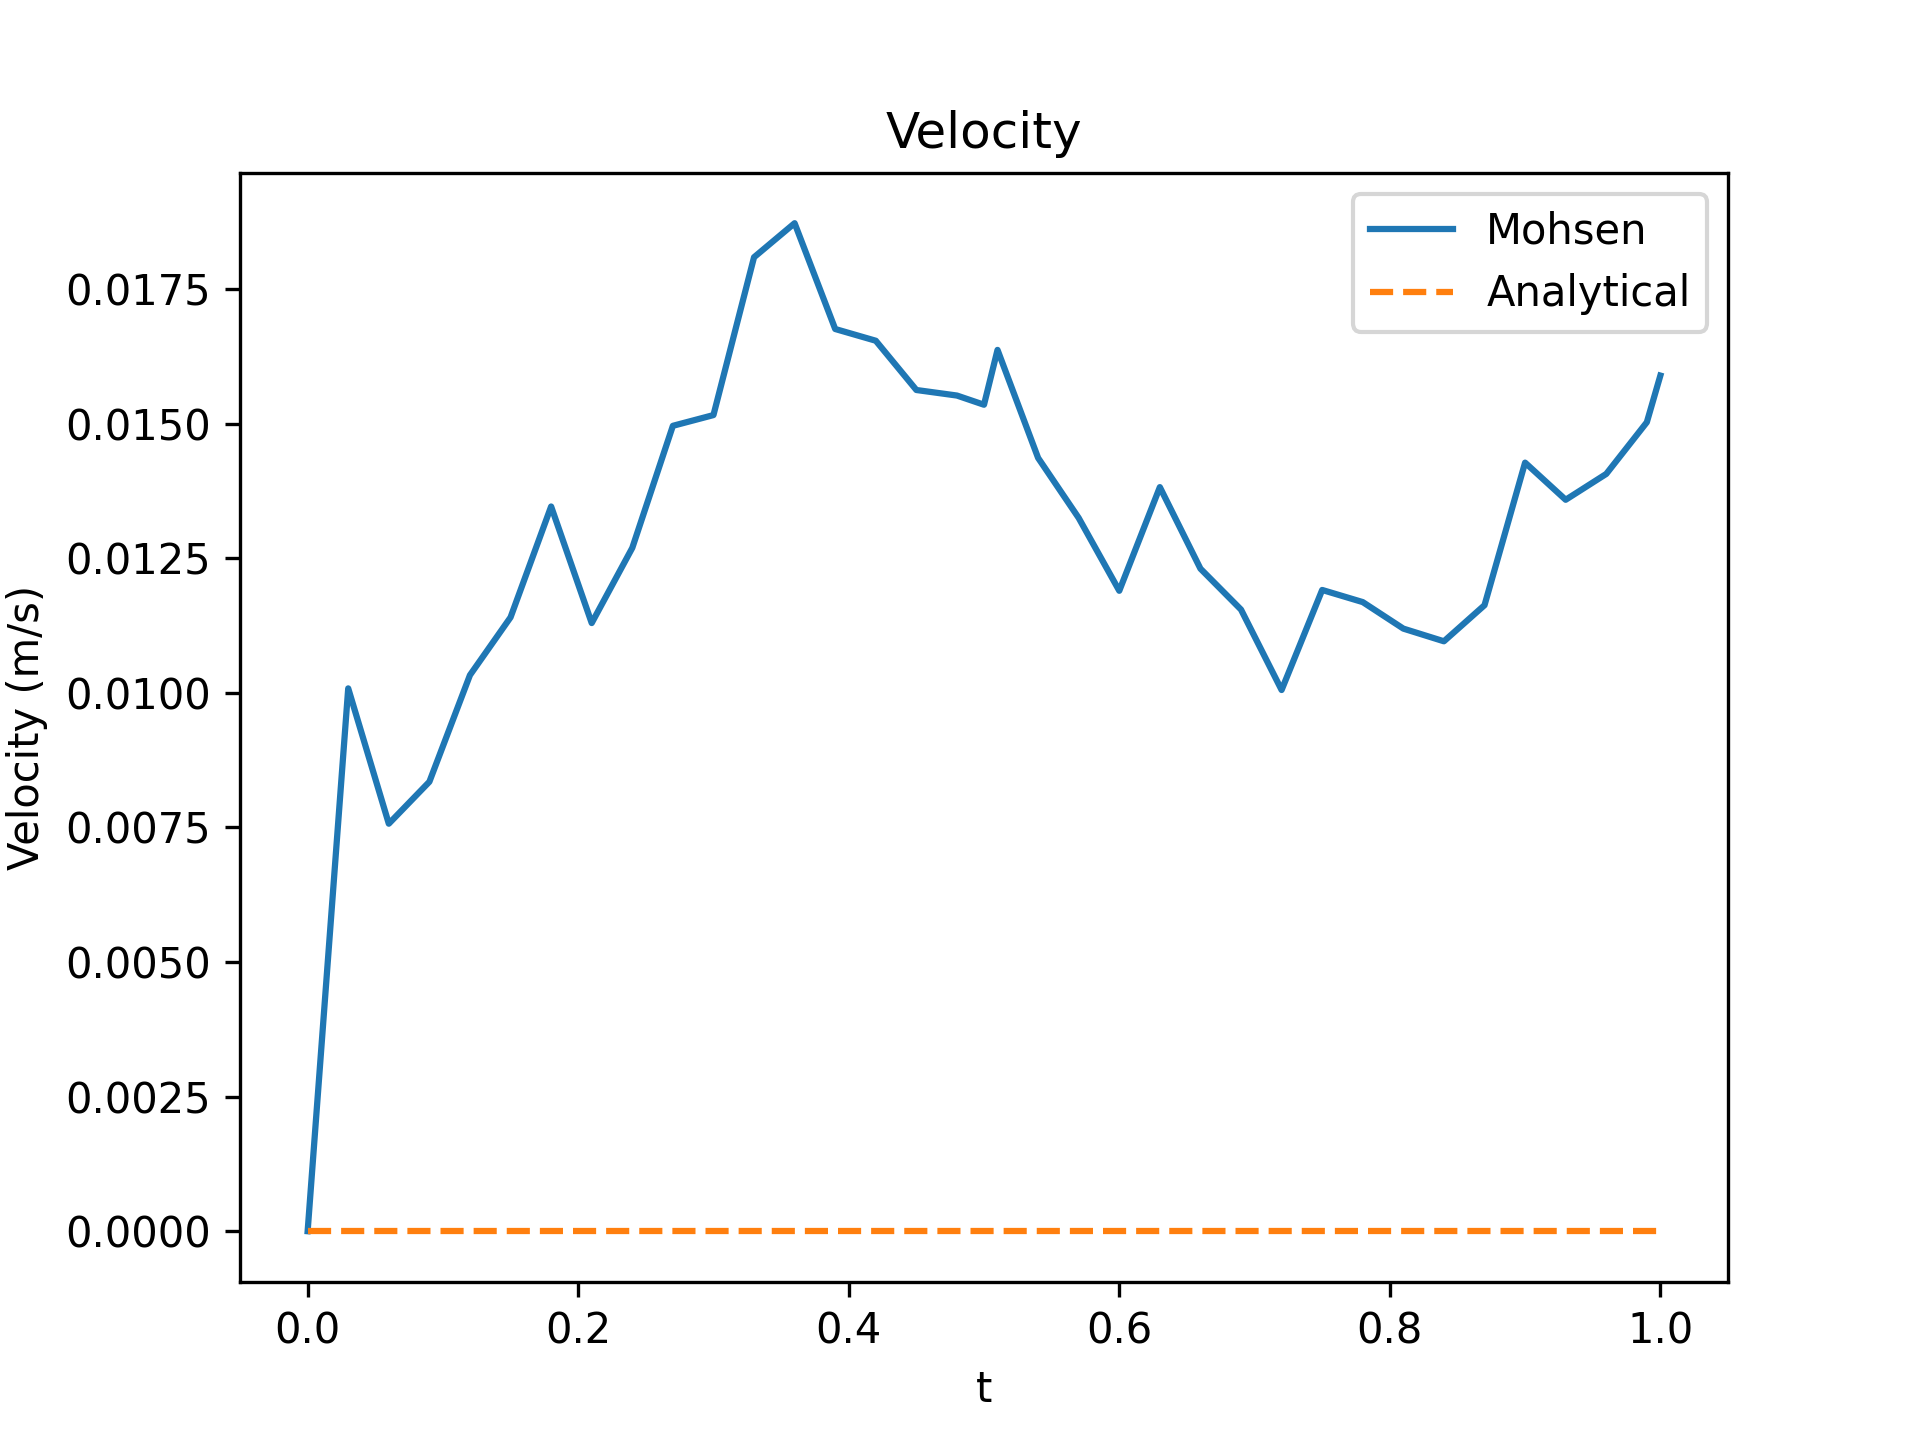
\includegraphics[width=0.6\textwidth]{figures/rfc/figures/mohseni_2021_free_sliding_on_a_slope_2d/velocity_vs_time}
  \caption{Variation of the velocity of the rigid body with time for different
    friction coefficients. Present result is compared against the analytical
    result.}
\label{fig:results-solid-sliding-velocity-vs-time-2d}
\end{figure}


% https://www.sciencedirect.com/science/article/pii/S0997754621001412#fig2
We study the behavior of a circular cylinder of density $500$
kg\,m\textsuperscript{-3} immersed in a hydrostatic tank under gravity. Since
the density of the solid body is half of the fluid, the body will be half afloat
while coming to rest. \Cref{fig:snapshots-rising-solid-in-water} presents
snapshot of a rising cylinder at time $t=15$ s and time variation of the center
of mass with time. As can be seen from the figure, since the density of the
cylinders is 500 kg\,m\textsuperscript{-3} the cylinder floats at half of its
diameter.
\begin{figure}[tpb]
  \centering
    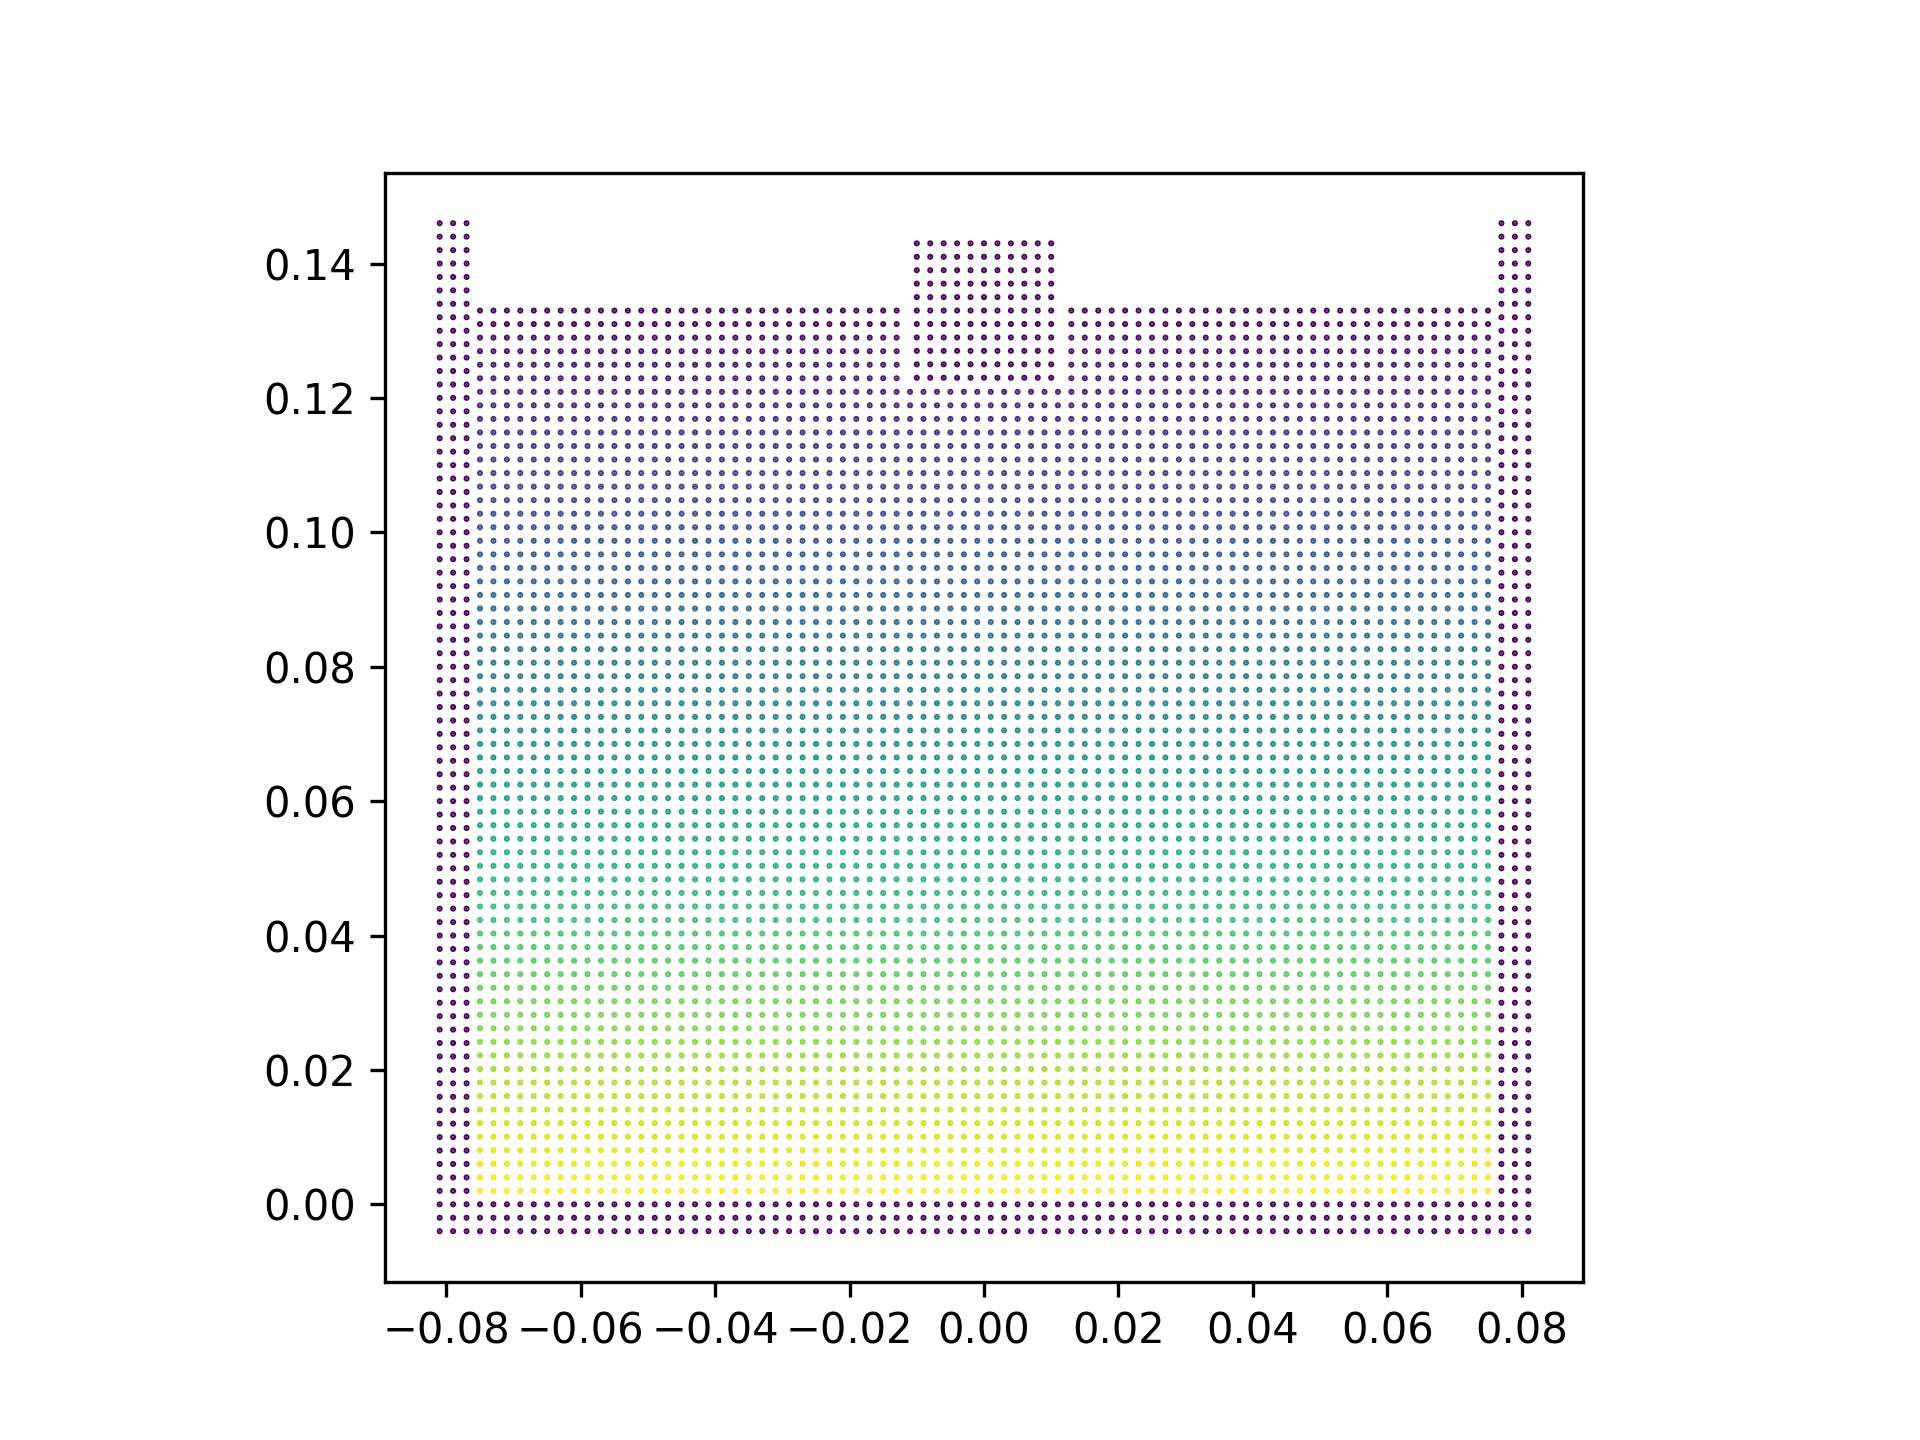
\includegraphics[width=0.4\textwidth]{images/rfc/images/water_entry_of_sphere/schematic}
  \caption{The schematic of an immersed cylinder in a hydrostatic tank.}
\label{fig:raising-falling-solid-in-water}
\end{figure}

\begin{figure}[tpb]
  \centering
  \begin{subfigure}{0.48\textwidth}
    \centering
    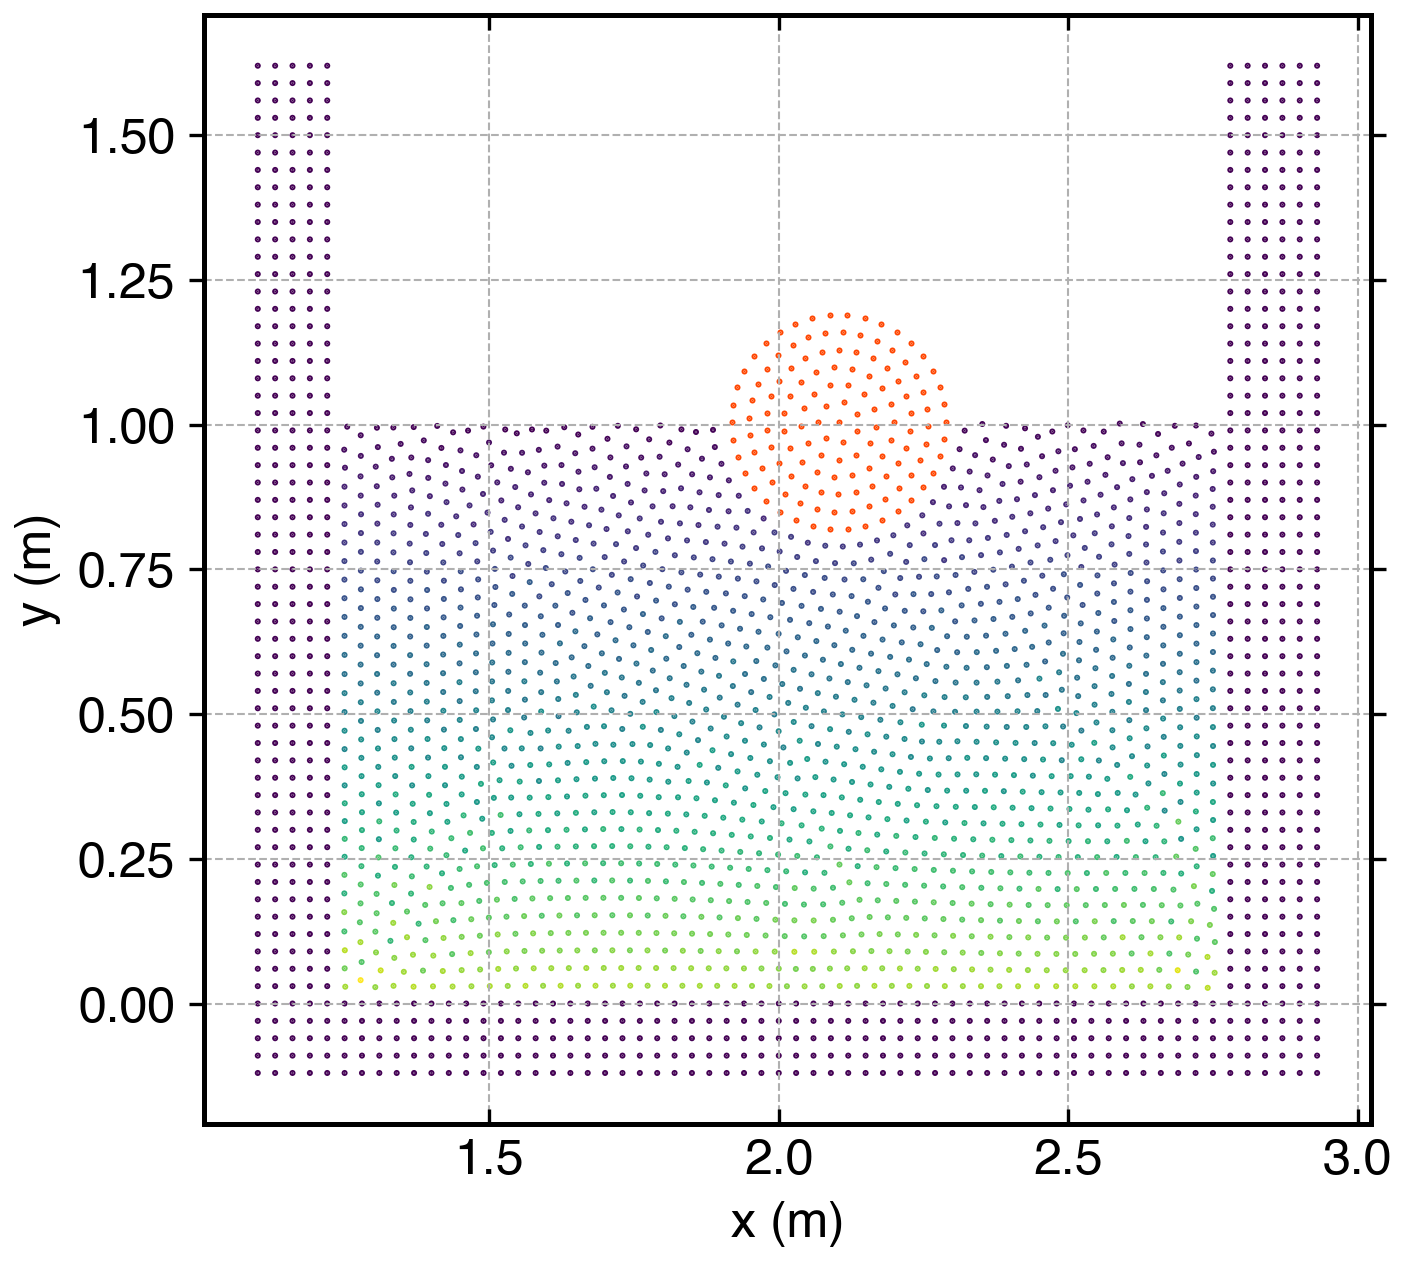
\includegraphics[width=1.0\textwidth]{figures/rfc/figures/dinesh_2022_body_in_hs_tank_2d/time11}
  \end{subfigure}
  %
  \begin{subfigure}{0.48\textwidth}
    \centering
    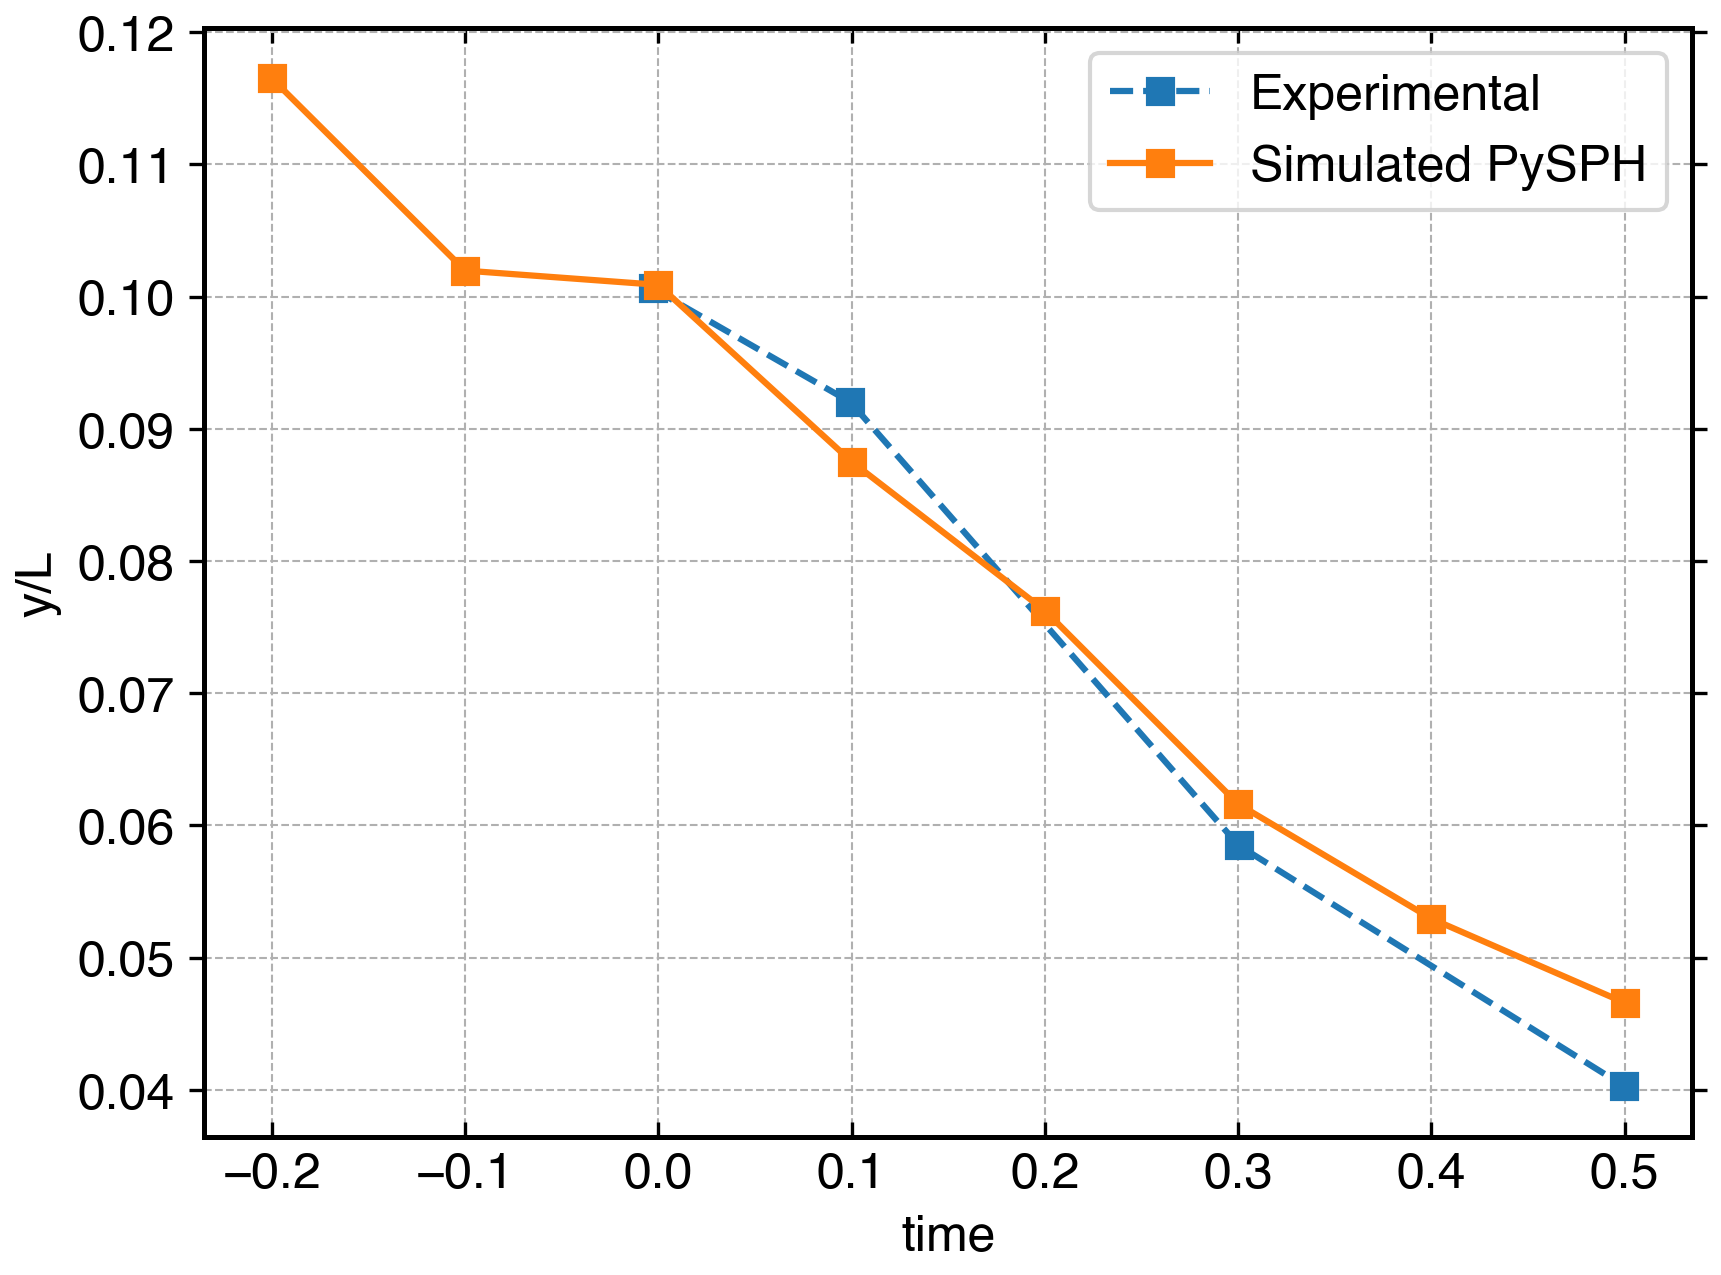
\includegraphics[width=1.0\textwidth]{figures/rfc/figures/dinesh_2022_body_in_hs_tank_2d/ycom}
  \end{subfigure}
  \caption{
    On the left, a snapshot at $t=15$ s is shown. On the right,
    time variation of the center of mass is shown.}
\label{fig:snapshots-rising-solid-in-water}
\end{figure}
